%========================================
% DETAILED SOLUTIONS: Funciones
%========================================

\subsection*{Ejercicio 1: Identificación de Funciones}

\textbf{Problema 1:} $\{(2,5), (3,7), (4,5), (5,9)\}$

\textbf{Solución detallada:}

Para determinar si una relación es función, verificamos que cada valor de entrada (primera coordenada) aparezca \textbf{exactamente una vez}.

\begin{itemize}
    \item Entrada 2 $\to$ Salida 5 \quad $\checkmark$
    \item Entrada 3 $\to$ Salida 7 \quad $\checkmark$
    \item Entrada 4 $\to$ Salida 5 \quad $\checkmark$
    \item Entrada 5 $\to$ Salida 9 \quad $\checkmark$
\end{itemize}

Cada entrada aparece solo una vez. El hecho de que 2 y 4 tengan la misma salida (5) \textbf{no viola} la definición de función. Lo que importa es que cada entrada tenga \textbf{una sola} salida.

\textbf{Respuesta:} SÍ es función.

\vspace{0.5cm}
\textbf{Problema 2:} $\{(-1,3), (0,5), (-1,7), (2,9)\}$

\textbf{Solución detallada:}

Examinamos cada entrada:
\begin{itemize}
    \item Entrada $-1$ $\to$ Salida 3
    \item Entrada 0 $\to$ Salida 5
    \item Entrada $-1$ $\to$ Salida 7 \quad \textcolor{red}{$\times$ PROBLEMA}
    \item Entrada 2 $\to$ Salida 9
\end{itemize}

El valor de entrada $-1$ aparece \textbf{dos veces} con salidas diferentes (3 y 7). Esto viola la definición de función.

\textbf{Respuesta:} NO es función.

\vspace{0.5cm}
\textbf{Problema 3:} $\{(a,1), (b,2), (c,3), (d,4)\}$

\textbf{Solución detallada:}

Aunque las entradas son letras en lugar de números, el concepto es el mismo:
\begin{itemize}
    \item $a \to 1$ (única salida para $a$)
    \item $b \to 2$ (única salida para $b$)
    \item $c \to 3$ (única salida para $c$)
    \item $d \to 4$ (única salida para $d$)
\end{itemize}

Cada entrada tiene exactamente una salida.

\textbf{Respuesta:} SÍ es función.

%========================================
\subsection*{Ejercicio 2: Evaluación de Funciones}

Dada $f(x) = 3x^2 - 2x + 1$

\textbf{Problema 1:} $f(2)$

\textbf{Estrategia:} Sustituir $x = 2$ en cada lugar donde aparece $x$ en la fórmula.

\begin{align*}
f(2) &= 3(2)^2 - 2(2) + 1 && \text{Sustituir } x = 2\\
&= 3(4) - 4 + 1 && \text{Evaluar el exponente: } 2^2 = 4\\
&= 12 - 4 + 1 && \text{Multiplicar: } 3 \times 4 = 12\\
&= 9 && \text{Simplificar}
\end{align*}

\vspace{0.5cm}
\textbf{Problema 2:} $f(-1)$

\textbf{Nota importante:} Cuando sustituimos un número negativo, debemos usar paréntesis.

\begin{align*}
f(-1) &= 3(-1)^2 - 2(-1) + 1 && \text{Sustituir } x = -1\\
&= 3(1) - 2(-1) + 1 && \text{Exponente: } (-1)^2 = 1\\
&= 3 + 2 + 1 && \text{Multiplicar: } -2 \times (-1) = +2\\
&= 6 && \text{Sumar}
\end{align*}

\vspace{0.5cm}
\textbf{Problema 3:} $f(0)$

Cuando evaluamos en cero, muchos términos se simplifican:

\begin{align*}
f(0) &= 3(0)^2 - 2(0) + 1\\
&= 3(0) - 0 + 1\\
&= 0 - 0 + 1\\
&= 1
\end{align*}

Este resultado nos dice que el intercepto en $y$ de la función es 1.

\vspace{0.5cm}
\textbf{Problema 4:} $f(a-1)$

\textbf{Estrategia:} Sustituir $x = (a-1)$ y expandir cuidadosamente.

\begin{align*}
f(a-1) &= 3(a-1)^2 - 2(a-1) + 1 && \text{Sustituir } x = a-1\\
&= 3(a^2 - 2a + 1) - 2a + 2 + 1 && \text{Expandir: } (a-1)^2\\
&= 3a^2 - 6a + 3 - 2a + 2 + 1 && \text{Distributiva}\\
&= 3a^2 + (-6a - 2a) + (3 + 2 + 1) && \text{Agrupar términos}\\
&= 3a^2 - 8a + 6 && \text{Simplificar}
\end{align*}

%========================================
\subsection*{Ejercicio 3: Función Lineal — Evaluación y Gráfica}

Dada $f(x) = 2x - 3$

\textbf{Problema 1:} Evaluar para $x = -1, 0, 1, 2$

\textbf{Estrategia:} Sustituir cada valor de $x$ en la función.

\begin{align*}
f(-1) &= 2(-1) - 3 = -2 - 3 = -5\\
f(0) &= 2(0) - 3 = 0 - 3 = -3\\
f(1) &= 2(1) - 3 = 2 - 3 = -1\\
f(2) &= 2(2) - 3 = 4 - 3 = 1
\end{align*}

\vspace{0.5cm}
\textbf{Problema 2:} Interpretar como puntos

Cada evaluación $f(a) = b$ genera el punto $(a, b)$:

\begin{center}
\begin{tabular}{|c|c|c|}
\hline
$x$ & $f(x)$ & Punto $(x, y)$ \\
\hline
$-1$ & $-5$ & $(-1, -5)$ \\
$0$ & $-3$ & $(0, -3)$ \\
$1$ & $-1$ & $(1, -1)$ \\
$2$ & $1$ & $(2, 1)$ \\
\hline
\end{tabular}
\end{center}

\textbf{Conexión importante:} El punto $(0, -3)$ es el \textbf{intercepto en y} de la función (donde la recta cruza el eje $y$).

\vspace{0.5cm}
\textbf{Problema 3:} Graficar

Para graficar una función lineal:
\begin{enumerate}
    \item \textbf{Ubique los puntos} en el plano cartesiano
    \item \textbf{Trace una recta} que pase por todos los puntos
\end{enumerate}

\textbf{Verificación:} Los cuatro puntos deben estar perfectamente alineados porque $f(x) = 2x - 3$ es una función lineal.

\textbf{Características de la gráfica:}
\begin{itemize}
    \item \textbf{Pendiente:} $m = 2$ (el coeficiente de $x$)
    \item \textbf{Interpretación de la pendiente:} Por cada unidad que avanzamos a la derecha, la recta sube 2 unidades
    \item \textbf{Intercepto en $y$:} $(0, -3)$ (el término constante)
    \item \textbf{Dirección:} Como $m = 2 > 0$, la recta sube de izquierda a derecha (pendiente positiva)
\end{itemize}

\textbf{Patrón observado:} Note que entre puntos consecutivos:
\begin{align*}
\text{De } (-1,-5) \text{ a } (0,-3): &\quad \Delta x = 1, \, \Delta y = 2 && \text{(razón: } 2/1 = 2\text{)}\\
\text{De } (0,-3) \text{ a } (1,-1): &\quad \Delta x = 1, \, \Delta y = 2 && \text{(razón: } 2/1 = 2\text{)}\\
\text{De } (1,-1) \text{ a } (2,1): &\quad \Delta x = 1, \, \Delta y = 2 && \text{(razón: } 2/1 = 2\text{)}
\end{align*}

Este patrón constante confirma la pendiente $m = 2$.

%========================================
\subsection*{Ejercicio 4: Dominio de Funciones}

\textbf{Problema 1:} $f(x) = \dfrac{1}{x+5}$

\textbf{Concepto clave:} En una fracción, el denominador nunca puede ser cero (división por cero no está definida).

\textbf{Paso 1:} Identificar cuándo el denominador es cero:
$$x + 5 = 0 \quad \Rightarrow \quad x = -5$$

\textbf{Paso 2:} Excluir este valor del dominio.

\textbf{Dominio:} Todos los reales excepto $-5$, escrito como $(-\infty, -5) \cup (-5, \infty)$

\vspace{0.5cm}
\textbf{Problema 2:} $g(x) = \sqrt{x-7}$

\textbf{Concepto clave:} La raíz cuadrada (índice par) solo está definida para radicandos no negativos.

\textbf{Paso 1:} Establecer la desigualdad:
$$x - 7 \ge 0$$

\textbf{Paso 2:} Resolver:
$$x \ge 7$$

\textbf{Dominio:} $[7, \infty)$

\textbf{Interpretación:} Solo podemos evaluar la función para valores de $x$ mayores o iguales a 7.

\vspace{0.5cm}
\textbf{Problema 3:} $h(x) = \dfrac{\sqrt{x-5}}{x-7}$

\textbf{Concepto clave:} Esta función tiene \textbf{dos restricciones}:
\begin{enumerate}
    \item La raíz cuadrada requiere $x - 5 \ge 0$
    \item El denominador requiere $x - 7 \ne 0$
\end{enumerate}

\textbf{Paso 1:} Resolver la restricción del radical:
$$x - 5 \ge 0 \quad \Rightarrow \quad x \ge 5$$

\textbf{Paso 2:} Identificar el valor prohibido del denominador:
$$x - 7 \ne 0 \quad \Rightarrow \quad x \ne 7$$

\textbf{Paso 3:} Combinar ambas condiciones:
\begin{itemize}
    \item $x \ge 5$ (de la raíz)
    \item $x \ne 7$ (del denominador)
\end{itemize}

Esto significa: $x$ puede ser cualquier valor desde 5 en adelante, \textbf{excepto} 7.

\textbf{Dominio:} $[5, 7) \cup (7, \infty)$

Visualmente en la recta numérica:
\begin{center}
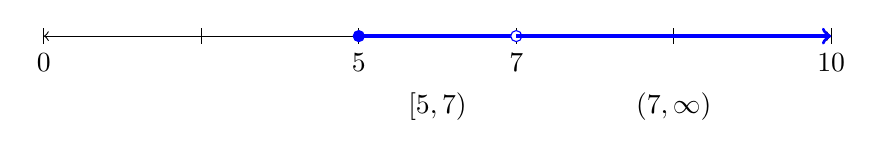
\begin{tikzpicture}
    \draw[<->] (0,0) -- (10,0);
    \foreach \x in {0,2,4,6,8,10}
        \draw (\x,0.1) -- (\x,-0.1);
    \node[below] at (0,-0.1) {0};
    \node[below] at (4,-0.1) {5};
    \node[below] at (6,-0.1) {7};
    \node[below] at (10,-0.1) {10};

    % Domain from 5 to 7 (not including 7)
    \draw[very thick, blue] (4,0) -- (6,0);
    \filldraw[blue] (4,0) circle (2pt); % Included
    \draw[blue, fill=white] (6,0) circle (2pt); % Not included

    % Domain from 7 to infinity
    \draw[very thick, blue, ->] (6,0) -- (10,0);

    \node[below] at (5,-0.6) {$[5, 7)$};
    \node[below] at (8,-0.6) {$(7, \infty)$};
\end{tikzpicture}
\end{center}

\vspace{0.5cm}
\textbf{Problema 4:} $k(x) = 5x - 3$

\textbf{Concepto clave:} Esta es una función lineal (polinomio de grado 1).

\textbf{Regla general:} Todas las funciones polinomiales tienen dominio de todos los números reales porque:
\begin{itemize}
    \item No hay división (sin problemas de denominador cero)
    \item No hay raíces pares (sin problemas de radicandos negativos)
\end{itemize}

\textbf{Dominio:} $(-\infty, \infty)$ o $\mathbb{R}$

%========================================
\subsection*{Ejercicio 5: Problemas Mixtos}

\textbf{Problema 1:} ¿La gráfica de $x^2 + y^2 = 16$ representa una función?

\textbf{Análisis completo:}

Esta ecuación representa un círculo con:
\begin{itemize}
    \item Centro en $(0, 0)$
    \item Radio $r = 4$ (porque $r^2 = 16$)
\end{itemize}

\textbf{Aplicando la prueba de la recta vertical:}

Consideremos la recta vertical $x = 0$ (el eje $y$):
\begin{align*}
(0)^2 + y^2 &= 16\\
y^2 &= 16\\
y &= \pm 4
\end{align*}

Esta recta interseca el círculo en \textbf{dos puntos}: $(0, 4)$ y $(0, -4)$.

\textbf{Conclusión:} Como existe al menos una recta vertical que interseca la gráfica en más de un punto, la relación \textbf{NO es función}.

\textbf{Intuición:} Para que el círculo fuera una función, cada valor de $x$ debería corresponder a un solo valor de $y$. Pero en un círculo, la mayoría de los valores de $x$ tienen dos valores de $y$ correspondientes (uno arriba y uno abajo).

\vspace{0.5cm}
\textbf{Problema 2:} Dada $f(x) = |x + 2|$

\textbf{a) Vértice:}

El vértice de una función de valor absoluto $f(x) = |x - h| + k$ está en $(h, k)$.

En nuestra función: $f(x) = |x - (-2)| + 0$

Por lo tanto: $h = -2$, $k = 0$

\textbf{Vértice:} $(-2, 0)$

\textbf{Verificación:} En $x = -2$: $f(-2) = |-2 + 2| = |0| = 0$ $\checkmark$

\textbf{b) Dominio:}

Las funciones de valor absoluto pueden evaluar cualquier número real.

\textbf{Dominio:} $(-\infty, \infty)$

\textbf{c) Rango:}

El valor absoluto siempre produce valores $\ge 0$. Como el vértice está en $y = 0$ y la función abre hacia arriba:

\textbf{Rango:} $[0, \infty)$

\vspace{0.5cm}
\textbf{Problema 3:} $f(x) = \sqrt{x+3}$

\textbf{Dominio:}
$$x + 3 \ge 0 \quad \Rightarrow \quad x \ge -3$$

\textbf{Dominio:} $[-3, \infty)$

\textbf{Punto inicial:} Cuando $x = -3$: $f(-3) = \sqrt{-3+3} = \sqrt{0} = 0$

El punto inicial es $(-3, 0)$.

\textbf{Puntos adicionales para graficar:}
\begin{itemize}
    \item $f(-2) = \sqrt{-2+3} = \sqrt{1} = 1$ $\to$ punto $(-2, 1)$
    \item $f(1) = \sqrt{1+3} = \sqrt{4} = 2$ $\to$ punto $(1, 2)$
    \item $f(6) = \sqrt{6+3} = \sqrt{9} = 3$ $\to$ punto $(6, 3)$
\end{itemize}

\vspace{0.5cm}
\textbf{Problema 4:} $g(x) = x^2 - 4$

\textbf{a)} $g(3) = (3)^2 - 4 = 9 - 4 = 5$

\textbf{b) Ceros de la función:}

Resolver $g(x) = 0$:
\begin{align*}
x^2 - 4 &= 0\\
x^2 &= 4\\
x &= \pm 2
\end{align*}

O usando factorización:
\begin{align*}
x^2 - 4 &= 0\\
(x-2)(x+2) &= 0\\
x = 2 &\text{ o } x = -2
\end{align*}

\textbf{Ceros:} $x = -2$ y $x = 2$

\textbf{c) Vértice:}

Para una parábola $f(x) = ax^2 + bx + c$:
$$x_{\text{vértice}} = -\frac{b}{2a}$$

En $g(x) = x^2 + 0x - 4$: $a = 1$, $b = 0$, $c = -4$
$$x_{\text{vértice}} = -\frac{0}{2(1)} = 0$$

Evaluar en $x = 0$:
$$g(0) = (0)^2 - 4 = -4$$

\textbf{Vértice:} $(0, -4)$

\textbf{Interpretación geométrica:} La parábola:
\begin{itemize}
    \item Abre hacia arriba (porque $a = 1 > 0$)
    \item Tiene su punto más bajo en $(0, -4)$
    \item Cruza el eje $x$ en $x = -2$ y $x = 2$
    \item Cruza el eje $y$ en $y = -4$
\end{itemize}
